\subsection{Metodo di Regolarizzazione di Tikhonov}
Per ridurre gli effetti del rumore nella ricostruzione è necessario introdurre un termine di regolarizzazione di Tikhonov. 

Si considera quindi il seguente problema di ottimizzazione:

Si deve risolvere $Ax_\epsilon = b_\epsilon$ con $b_\epsilon = b+\epsilon$. 
Al posto di risolvere direttamente il sistema lineare (se il sistema è quadrato) o di minimizzare la norma 2 del residuo 
(se il sistema è rettangolare)  $||Ax_\epsilon -b_\epsilon||_2^2$, %! davvero dobbiamo mettere la formula?!

si aggiunge un vincolo di regolarità alla soluzione e si minimizza, ad esempio 
\[||Ax_\epsilon-b_\epsilon||_2^2+\gamma_\epsilon||x_\epsilon||_2^2\] che rappresenta la \textbf{forma standard} 
della regolarizzazione di Tikhonov.

Analizziamo i grafici ottenuti cercando di ridurre il rumore nella ricostruzione delle immagini del dataset. 
\begin{figure}[H]
    \centering
    \begin{subfigure}{0.5\textwidth}
        \centering
        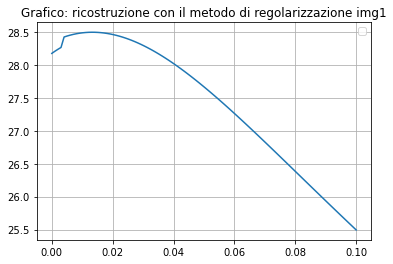
\includegraphics[width=\textwidth]{output/PSNR/outputPSNR-img1.png}
        \caption{PSNR di img1}
        \label{fig:img1PSNR}
    \end{subfigure}\hfill
    \begin{subfigure}{0.5\textwidth}
        \centering
        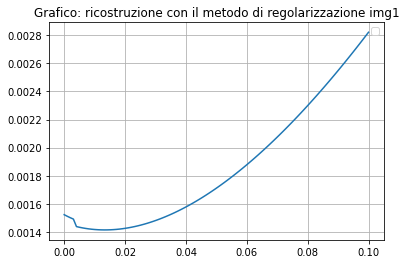
\includegraphics[width=\textwidth]{output/MSE/outputMSE-img1.png}
        \caption{MSE di img1}
        \label{fig:img1MSE}
    \end{subfigure}

    \begin{subfigure}{0.5\textwidth}
        \centering
        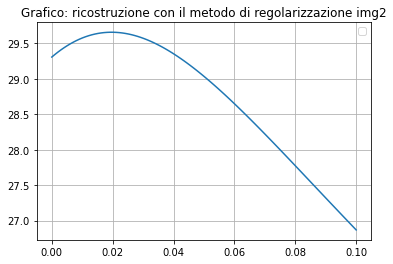
\includegraphics[width=\textwidth]{output/PSNR/outputPSNR-img2.png}
        \caption{PSNR di img2}
        \label{fig:img2PSNR}
    \end{subfigure}\hfill
    \begin{subfigure}{0.5\textwidth}
        \centering
        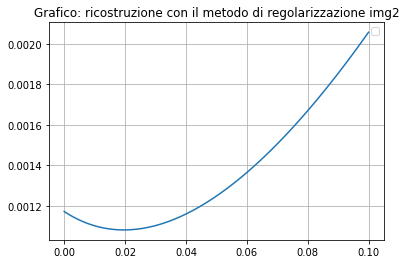
\includegraphics[width=\textwidth]{output/MSE/outputMSE-img2.png}
        \caption{MSE di img2}
        \label{fig:img2MSE}
    \end{subfigure}
    \caption{Grafici andamento PSNR e MSE nella ricostruzione delle immagini con il metodo di regolarizzazione}
\end{figure}%
\begin{figure}[H]\ContinuedFloat
    \centering
    \begin{subfigure}{0.5\textwidth}
        \centering
        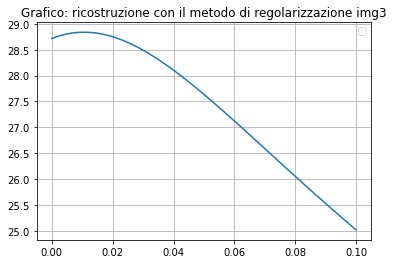
\includegraphics[width=\textwidth]{output/PSNR/outputPSNR-img3.png}
        \caption{PSNR di img3}
        \label{fig:img3PSNR}
    \end{subfigure}\hfill
    \begin{subfigure}{0.5\textwidth}
        \centering
        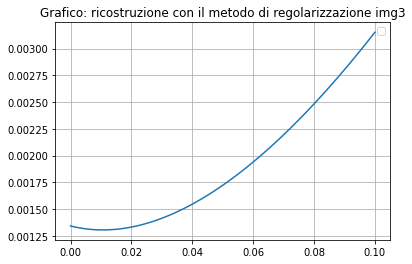
\includegraphics[width=\textwidth]{output/MSE/outputMSE-img3.png}
        \caption{MSE di img3}
        \label{fig:img3MSE}
    \end{subfigure}

    \begin{subfigure}{0.5\textwidth}
        \centering
        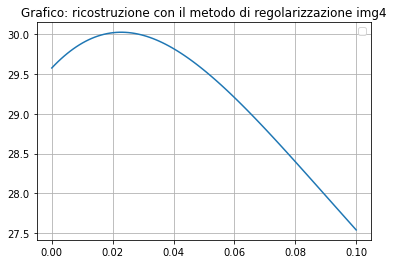
\includegraphics[width=\textwidth]{output/PSNR/outputPSNR-img4.png}
        \caption{PSNR di img4}
        \label{fig:img4PSNR}
    \end{subfigure}\hfill
    \begin{subfigure}{0.5\textwidth}
        \centering
        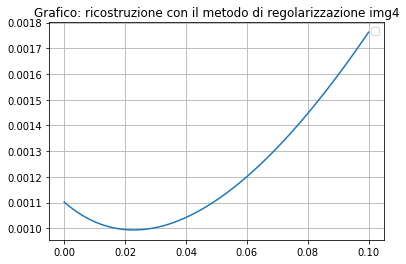
\includegraphics[width=\textwidth]{output/MSE/outputMSE-img4.png}
        \caption{MSE di img4}
        \label{fig:img4MSE}
    \end{subfigure}

    \begin{subfigure}{0.5\textwidth}
        \centering
        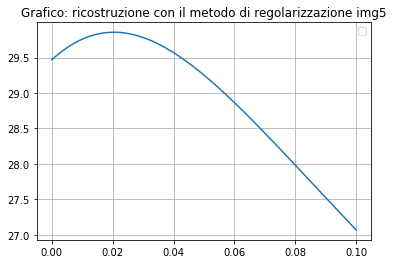
\includegraphics[width=\textwidth]{output/PSNR/outputPSNR-img5.png}
        \caption{PSNR di img5}
        \label{fig:img5PSNR}
    \end{subfigure}\hfill
    \begin{subfigure}{0.5\textwidth}
        \centering
        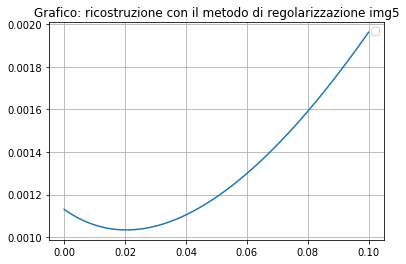
\includegraphics[width=\textwidth]{output/MSE/outputMSE-img5.png}
        \caption{MSE di img5}
        \label{fig:img5MSE}
    \end{subfigure}

    \begin{subfigure}{0.5\textwidth}
        \centering
        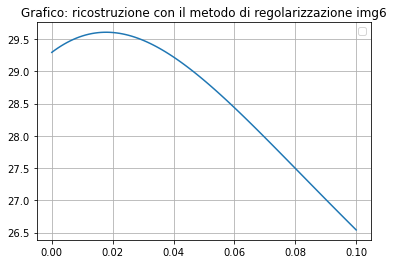
\includegraphics[width=\textwidth]{output/PSNR/outputPSNR-img6.png}
        \caption{PSNR di img6}
        \label{fig:img6PSNR}
    \end{subfigure}\hfill
    \begin{subfigure}{0.5\textwidth}
        \centering
        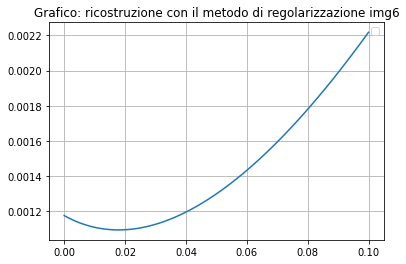
\includegraphics[width=\textwidth]{output/MSE/outputMSE-img6.png}
        \caption{MSE di img6}
        \label{fig:img6MSE}
    \end{subfigure}
    \caption{Grafici andamento PSNR e MSE nella ricostruzione delle immagini con il metodo di regolarizzazione}
\end{figure}%
\begin{figure}[H]\ContinuedFloat
    \centering
    \begin{subfigure}{0.5\textwidth}
        \centering
        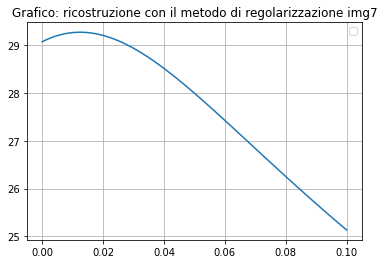
\includegraphics[width=\textwidth]{output/PSNR/outputPSNR-img7.png}
        \caption{PSNR di img7}
        \label{fig:img7PSNR}
    \end{subfigure}\hfill
    \begin{subfigure}{0.5\textwidth}
        \centering
        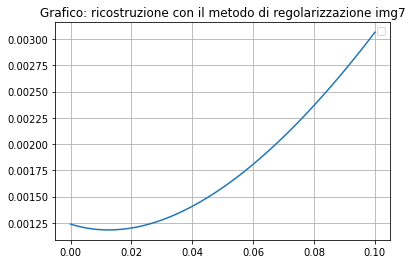
\includegraphics[width=\textwidth]{output/MSE/outputMSE-img7.png}
        \caption{MSE di img7}
        \label{fig:img7MSE}
    \end{subfigure}

    \begin{subfigure}{0.5\textwidth}
        \centering
        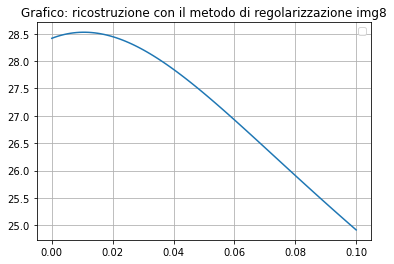
\includegraphics[width=\textwidth]{output/PSNR/outputPSNR-img8.png}
        \caption{PSNR di img8}
        \label{fig:img8PSNR}
    \end{subfigure}\hfill
    \begin{subfigure}{0.5\textwidth}
        \centering
        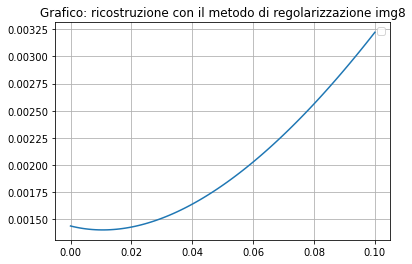
\includegraphics[width=\textwidth]{output/MSE/outputMSE-img8.png}
        \caption{MSE di img8}
        \label{fig:img8MSE}
    \end{subfigure}
\caption{Grafici andamento PSNR e MSE nella ricostruzione delle immagini con il metodo di regolarizzazione}
\end{figure}

Per quanto riguarda le immagini fotografiche, abbiamo riscontrato un curioso errore. 

\begin{figure}[H]
    \centering
    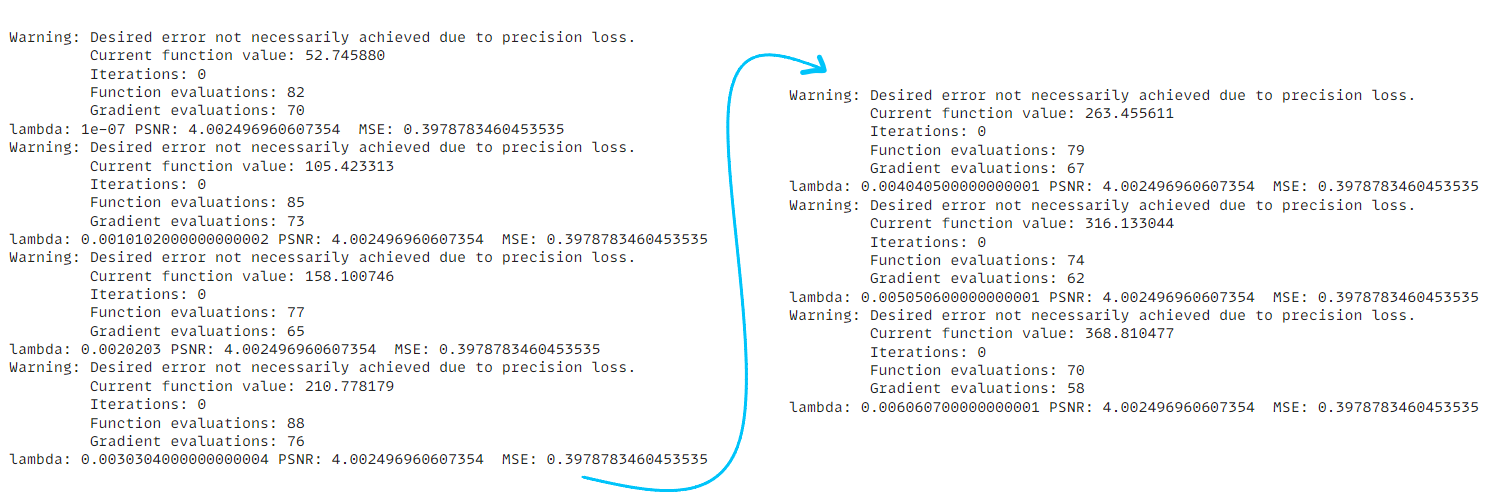
\includegraphics[width=\textwidth]{output/outputERROR.png}
    \caption{Errore immagini fotografiche}
    \label{fig:errorOutput}
\end{figure}

Possiamo affermare che l'incremento è talmente impercettibile che non viene colto dal calcolatore poiché inferiore alla sua precisione macchina, con la regolarizzazione si ottengono comunque risultati migliori. 
